\documentclass{article}

\usepackage{amsmath}
\usepackage{tikz}
\usepackage{graphicx}

\title{Turing Machine Documentation}
\author{Ryan Peruski, Maria Hernandez}
\date{\today}

\begin{document}

\maketitle
\section{Roles}

\begin{itemize}
    \item Ryan Peruski: Created initial stack design and initial templates for the documentation
    \item Maria Hernandez
\end{itemize}
\section{Definition}
This Turing machine uses the power of the stack to do a simple check for C-code. It checks for correct parenthesis, square bracket, and curly brace
placement. It will accept any code that has correct placement of these characters, and it will reject any code that does not.

\section{States, Transitions, Image}
The Turing machine operates by moving between states and performing transitions on the tape. The states and transitions are labelled as follows:

\begin{itemize}
    \item $Red$ are all the reject states ($q_{reject}$)
    \item $Green$ are all the accept states ($q_{accept}$)
    \item $Blue$ is the Queue's add States
    \item $Yellow$ is the Queue's remove States (1st part: $deletion$)
    \item $Orange$ is the Queue's remove States  (2nd part: $movement$)
    \item $Magenta$ is the Stack with the add states
    \item $Cyan$ is the Stack with the remove states
    \item $Black$ are the initial states to set up the $\#$
    \item $Beige$ transition states to go to either stack or queue / validity of the string
\end{itemize}

The transitions can be summarized as follows:
\begin{itemize}
    \item xxxxxx
    \item xxxxxx
\end{itemize}

Finally, the Turing Machine is shown in Figure\ \ref{fig:stackqueue}.
\begin{figure}
    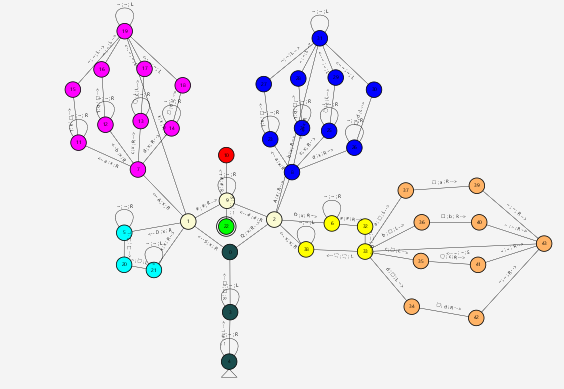
\includegraphics[width=\linewidth]{stackqueue.png}
    \caption{Turing Machine.}\label{fig:stackqueue}
\end{figure}

\section{Instructions}
This Turing Machine can input any C-code (or code in general that uses parenthesis) and it will place left parenthesis on the stack and pop
right parenthesis. If it does not see a parenthesis of the right type or none at all, it will reject. If the code ends with anything on the
stack, it will reject. If the code is empty, it will accept. 

The only thing that the machine will reject on is a $\#$, as this is a marker between the code and the stack.

Note that machine CANNOT handle whitespace ANYWHERE
Also, when using a backslash within quotes, only the quotes, newlines, and null characters are accepted.
Of course, we could add more support for backslash characters, but we didn't want to make the machine too needlessly complicated.

\section{Examples}
Here are some examples of input and output for the Turing machine:
\begin{itemize}
    \item \begin{verbatim} Input: v[i]=a[i][j];, Output:  xxxxxxxxxxxxx#bqa \end{verbatim}
    \item \begin{verbatim} Input: for(;;)break;, Output:  xxxxxxxxxxxxx#bqa \end{verbatim}
    \item \begin{verbatim} Input: {x=7}, Output: xxxxx#bqa \end{verbatim}
    \item \begin{verbatim} Input: for(i=0;i<v.size();i++)v[i]=2;, Output: xxxxxxxxxxxxxxxxxxxxxxxxxxxxxx#bqa \end{verbatim}
    \item \begin{verbatim} Input: v[i]=a[i, Output:  xxxxxxxx#Rqr \end{verbatim}
    \item \begin{verbatim} Input: for(;;, Output:  xxxxxx#Rqr \end{verbatim}
    \item \begin{verbatim} Input: printf("HelloWorld!\n");, Output:   xxxxxxxxxxxxxxxxxxxxxxxx#bqa \end{verbatim}
    \item \begin{verbatim} Input: printf("Hereisa{(");, Output:  xxxxxx#qa\end{verbatim}
    \item \begin{verbatim} Input: """, Output: xxx#qr\end{verbatim}
    \item \begin{verbatim} Input: 'a''\n', Output: xxxxxxx#bqa\end{verbatim}
    \item \begin{verbatim} Input: /*WeSupportComments!*/, Output:  xxxxxxxxxxxxxxxxxxxxxx#bqa \end{verbatim}
    \item \begin{verbatim} Input: /*WeSupportComments!{{{{*/, Output:  xxxxxxxxxxxxxxxxxxxxxxxxxx#bqa \end{verbatim}
    \item \begin{verbatim} Input: /*/*/, Output: xxxxx# , ACCEPTS \end{verbatim}  
    \item \begin{verbatim} Input: /*/*, Output: xxxx#/* , REJECTS \end{verbatim}
    \item \begin{verbatim} Input: */*/, Output:  xx*/#  , REJECTS \end{verbatim}
    \item \begin{verbatim} Input: /*a*b*/, Output: xxxxxxx# , ACCEPTS \end{verbatim}
    \item \begin{verbatim} Input: /*HelloWorld*/*/, Output: xxxxxxxxxxxxxxxx#  , REJECTS \end{verbatim}
    \item \begin{verbatim} Input: /*/**/, Output:  xxxxxx# , ACCEPTS, NOTE: It accepts because it treats the inner /* as comment, but normal compilers throw a warning in these cases \end{verbatim} 
    \item \begin{verbatim} Input: /*}*/, Output: xxxxx# , ACCEPTS, NOTE: } doesn't have the opening {, but this accepts because it treats anything inside /**/ as comments \end{verbatim}
    \item \begin{verbatim} Input: /*/**/*/, Output: xxxxxxxx# , REJECTS, NOTE: last */ does not have an opening /*. Compilers do not accept nested comments \end{verbatim}
    \item \begin{verbatim} Input: /*a*b* , Output: xxxxxx#/*  , REJECTS \end{verbatim}
    \item \begin{verbatim} Input: (/, Output:  xx#( , REJECTS \end{verbatim} 
    \item \begin{verbatim} Input: (/*****)*/* , Output:  xxxxxxxxxxx#( , REJECTS, NOTE: needs closing ) \end{verbatim}
    \item \begin{verbatim} Input: (/*****)*/*), Output:  xxxxxxxxxxxx# , ACCEPTS \end{verbatim}
    \item \begin{verbatim} Input: (/*****)*/*)*, Output:  xxxxxxxxxxxxx# , ACCEPTS \end{verbatim}
    \item \begin{verbatim} Input: (/*)Hi***/}"", Output: xxxxxxxxxxx""#( , REJECTS, Note: rejects as soon as } doenst match ( \end{verbatim}
    \item \begin{verbatim} Input: *{/}, Output:  xxxx# , ACCEPTS \end{verbatim}
    \item \begin{verbatim} Input: /(*), Output:  xxxx# , ACCEPTS \end{verbatim}
    \item \begin{verbatim} Input: *(*), Output:  xxxx# , ACCEPTS \end{verbatim}
    \item \begin{verbatim} Input: *[/}, Output:  xxxx# , ACCEPTS \end{verbatim}

\end{itemize}

\section{Considerations} 
\begin{verbatim} 
The operators that gave us the most work were /* and */ since the tape reads one character at a time, we needed to take into account a lot of possible scenarios so that the machine 
does not halt, and correctly behaves when the original tape has something like *{/}, or /(*), or, *(*), or *[/} (reject in this case.). That's why there are a lot of transitions 
coming out of states 24 and 25. Also, we needed a special branch (purple branch) for the comments so that we could ignore everything inside /* */
\end{verbatim}
\section{Conclusion}
The Turing machine is a powerful tool for performing computations on input tapes. It has applications in computer science, mathematics, and other fields.


\end{document}


To do: 
- specify what's bad input and what's good input